\documentclass[12pt,letterpaper]{article}
\usepackage[utf8]{inputenc}
\usepackage[spanish]{babel}
\usepackage{graphicx}
\usepackage[left=2cm,right=2cm,top=2cm,bottom=2cm]{geometry}
\usepackage{graphicx} % figuras
% \usepackage{subfigure} % subfiguras
\usepackage{float} % para usar [H]
\usepackage{amsmath}
%\usepackage{txfonts}
\usepackage{stackrel} 
\usepackage{multirow}
\usepackage{enumerate} % enumerados
\renewcommand{\labelitemi}{$-$}
\renewcommand{\labelitemii}{$\cdot$}
% \author{}
% \title{Caratula}
\begin{document}

% Fancy Header and Footer
% \usepackage{fancyhdr}
% \pagestyle{fancy}
% \cfoot{}
% \rfoot{\thepage}
%

% \usepackage[hidelinks]{hyperref} % CREA HYPERVINCULOS EN INDICE

% \author{}
\title{Caratula}

\begin{titlepage}
\begin{center}
\large{UNIVERSIDAD PRIVADA DE TACNA}\\
\vspace*{-0.025in}
\begin{figure}[htb]
\begin{center}

\includegraphics[width=7cm]{./images/logo}
\end{center}
\end{figure}
\vspace*{0.15in}
INGENIERIA DE SISTEMAS  \\

\vspace*{0.3in}
\begin{large}
\textbf{TITULO:} \\
\end{large}

\vspace*{0.1in}
\begin{Large}
\textbf{Informe de Laboratorio 01} \\

\end{Large}

\vspace*{0.3in}
\begin{Large}
\textbf{CURSO:} \\
\end{Large}

\vspace*{0.1in}
\begin{large}
INTELIGENCIA DE NEGOCIOS\\
\end{large}

\vspace*{0.3in}
\begin{Large}
\textbf{DOCENTE:} \\
\end{Large}

\vspace*{0.1in}
\begin{large}
 Ing. Patrick Cuadros Quiroga\\
\end{large}

\vspace*{0.4in}
\vspace*{0.1in}
\begin{large}
\textbf{ESTUDIANTE:} \\
\begin{flushleft}
Anthony Robles Flores \hfill	(2016056192)\\

\centering  %CENTRA UN TEXTO
\vspace*{0.9in}
\begin{large}
Tacna
\end{large}

\end{flushleft}
\end{large}
\end{center}

\end{titlepage}


\tableofcontents % INDICE
\thispagestyle{empty} % INDICE SIN NUMERO
\newpage
\setcounter{page}{1} % REINICIAR CONTADOR DE PAGINAS DESPUES DEL INDICE


%%INICIO Resumen
\section{Onjetivos}
El objetivo final es que estos puedan encontrar de manera intuitiva y rápida la información que necesitan,analizar los datos que hacen referencia a hechos, sean económicos o de otros tipos, desde la perspectiva de sus componentes o dimensiones.
%%FIN Resumen


%%INICIO Introducción
\section{Requerimientos}
Conocimientos
\\
Para el desarrollo de esta práctica se requerirá de los siguientes conocimientos básicos:
	\begin{itemize}
	\item Conocimientos básicos de administración de base de datos Microsoft SQL Server.
	\item Conocimientos básicos de SQL.
	\end{itemize}

Software
\\
Asimismo se necesita los siguientes aplicativos:
	\begin{itemize}
	\item Microsoft SQL Server 2016 o superior
	\item Base de datos AdventureWorksDW2016 o superior
	\end{itemize}
%%FIN Introducción


%%INICIO Marco Teórico
\section{Consideraciones Iniciales}
Generar todos los modelos fisicos de los diagramas entidad relación y modelo dimensional en bases de datos
separadas en Microsoft SQL Server.

%%----------------------------------------------------------------------------------------------------------------------------------------------------------
%%INICIO Marco Teórico
\section{Desarrollo}

\subsection{\textbf{Ejercicio 01}}
El siguiente diagrama ER simplificado describe el envio de mercancias. Los lotes pertenecientes a ciertos grupos se
envian a ciertos destinos en varios paises a traves de diferentes modos de transporte. Un cierto centro de costos es
responsable de cada envio. La dimension de tiempo consiste en mes y anio.



%\section{EJERCICIO 01: Envíos} 

\textbf{MODELO FISICO}\\\\
\begin{center}
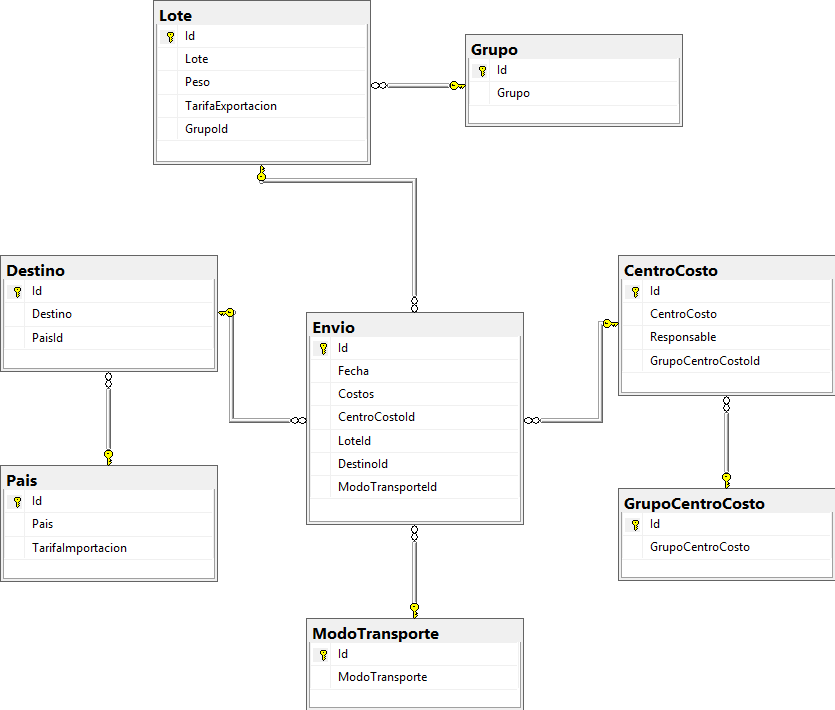
\includegraphics[width=\columnwidth]{images/task1/e1}\newline
\end{center}

\textbf{MODELO DIMENSIONAL}\\\\
\begin{center}
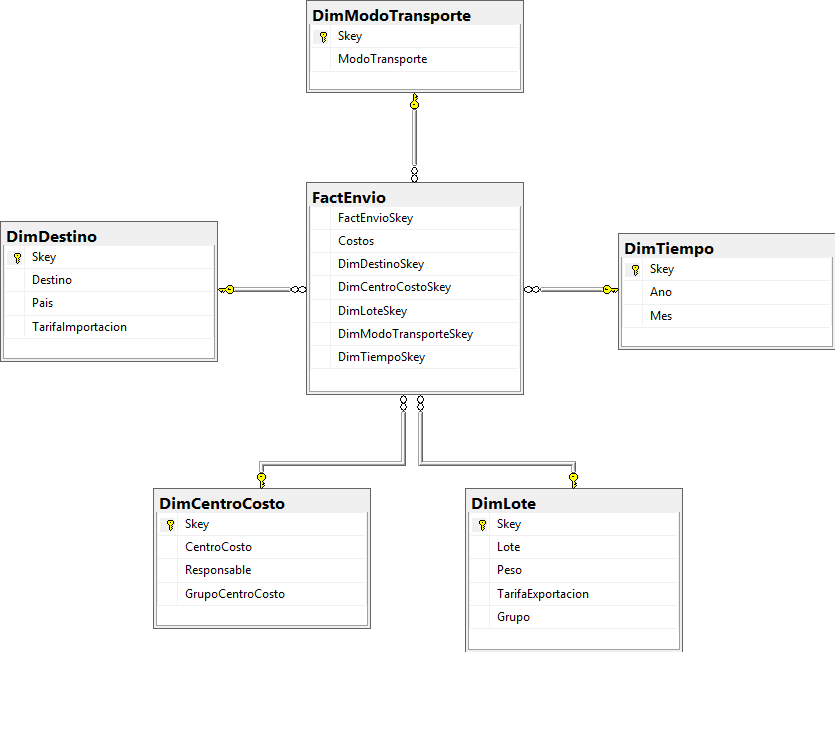
\includegraphics[width=\columnwidth]{images/task1/d1}\newline
\end{center}



\section{EJERCICIO 02: Reservas de viaje} 

\textbf{MODELO FISICO}\\\\
\begin{center}
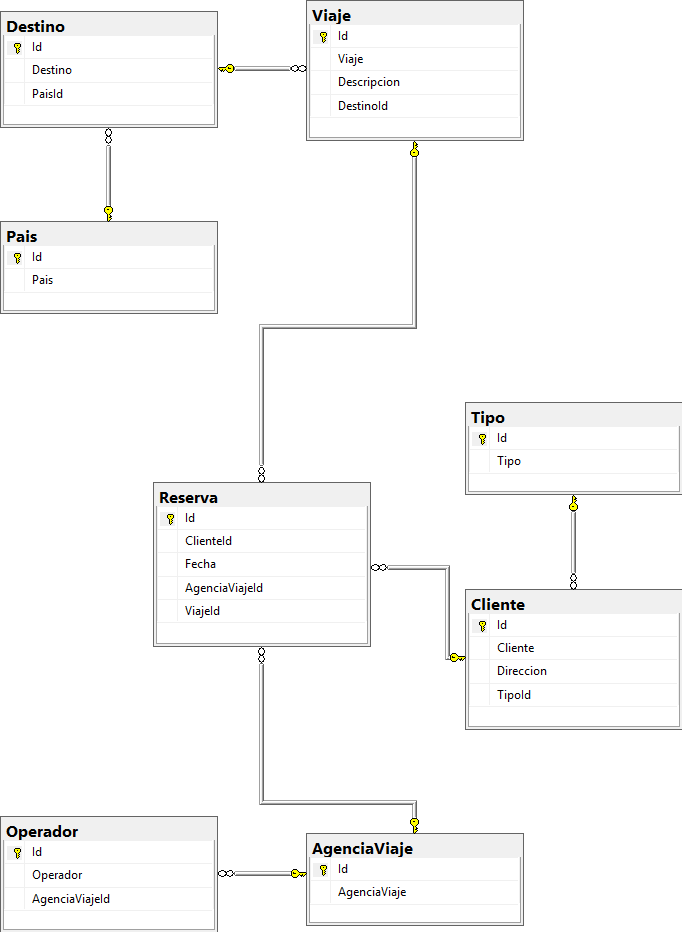
\includegraphics[width=\columnwidth]{images/task2/e2}\newline
\end{center}

\textbf{MODELO DIMENSIONAL}\\\\
\begin{center}
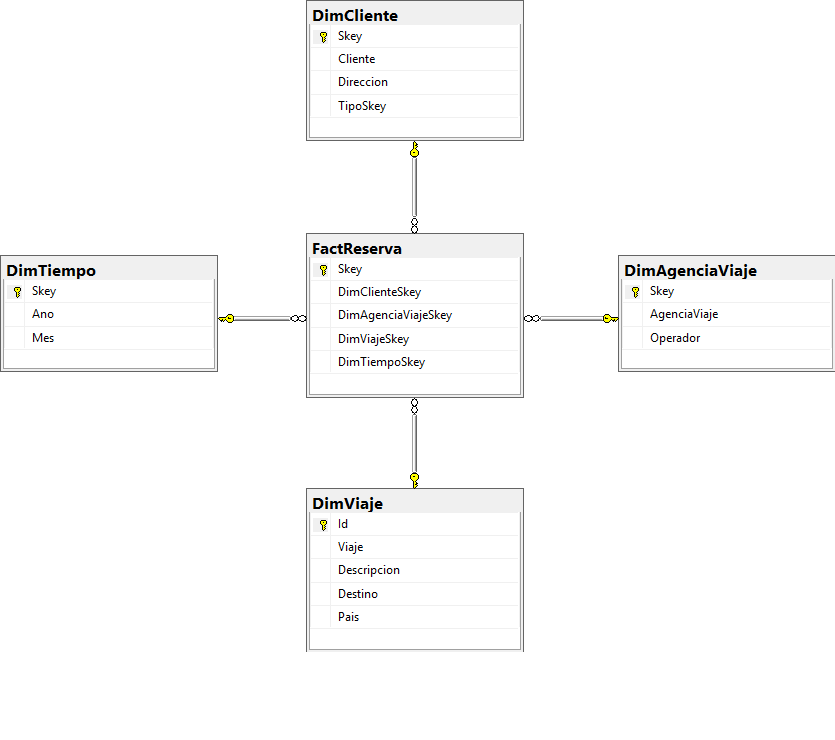
\includegraphics[width=\columnwidth]{images/task2/d2}\newline
\end{center}
\section{EJERCICIO 03: Gestión de proyectos } 

\textbf{MODELO FISICO}\\\\
\begin{center}
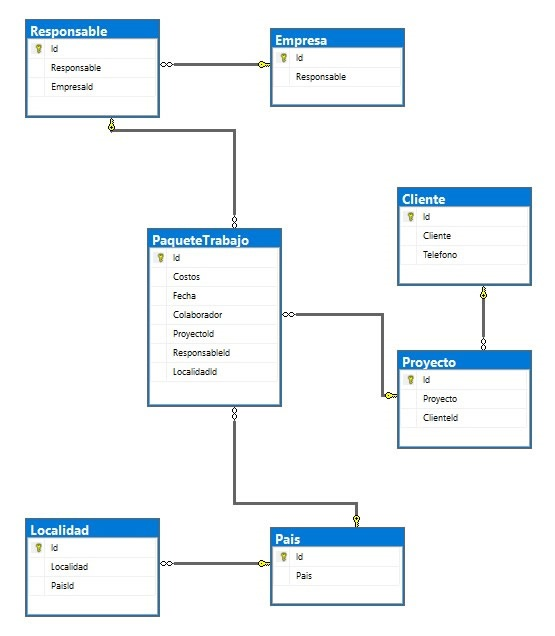
\includegraphics[width=\columnwidth]{images/task3/e3}\newline
\end{center}

\textbf{MODELO DIMENSIONAL}\\\\
\begin{center}
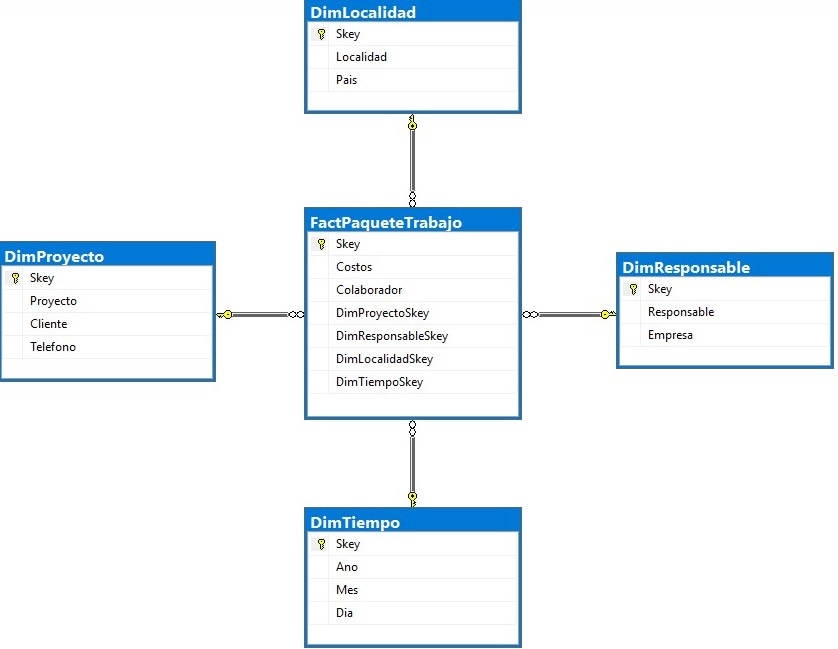
\includegraphics[width=\columnwidth]{images/task3/d3}\newline
\end{center}


\end{document}